\documentclass[11pt]{article}

\usepackage[a4paper,margin=2.2cm]{geometry}
\usepackage[T1]{fontenc}
\usepackage{lmodern}
\usepackage{microtype}
\usepackage{hyperref}
\usepackage{enumitem}
\emergencystretch=2em
\usepackage{booktabs}
\usepackage{tabularx}
\usepackage{array}
\usepackage{graphicx} % for \fbox/\parbox convenience (often already present)
\usepackage{tikz}
\usetikzlibrary{arrows.meta,positioning,calc}
\setlist[itemize]{leftmargin=*}
\setlist[enumerate]{leftmargin=*}
\setlist[description]{leftmargin=0pt,labelsep=0.6em,style=unboxed,itemsep=0.25\baselineskip}

\title{From Apps to Answers: Connecting Public Sector Data to AI with MCP\\
\large Research brief (working draft)}
\author{Chris Page}
\date{\today}

\begin{document}
\maketitle

\section*{Executive summary}

The UK public sector is rich in data (open data through to highly sensitive operational and personal data), but it is often \emph{hard to turn into answers}. \cite{oecd_data_driven_public_sector2019,nao_data_across_gov} Historically, we built applications as the primary interface to data, and trained people to use the applications.

This brief proposes a complementary model: \textbf{Apps $\rightarrow$ Answers}. In this model, people ask questions in plain language; an intelligence layer (increasingly AI) interprets intent; and a controlled ``middle layer'' transforms raw data into usable information with provenance, permissions, and auditability. \cite{mcp_spec_2025_11_25,prov_o,prov_dm}

The middle layer is where practical responsibility sits: (1) \textbf{dataset scoping and permissions}; (2) \textbf{discovery and semantics} (what data exists, what it means); (3) \textbf{provenance and audit} (how an answer was produced, and how to reproduce it); (4) \textbf{safety guardrails} (policy, privacy, and acceptable use); and (5) \textbf{operations} (cost, latency, reliability, and degradation). \cite{ncsc_secure_ai_guidelines,ico_ai_data_protection,data_ai_ethics_framework,five_safes_framework,algorithmic_transparency_recording_standard}

We use \textbf{Model Context Protocol (MCP)} and an example server (\textbf{MCP-Geo}, combining Ordnance Survey and Office for National Statistics data) to make this concrete: \emph{capabilities over applications}. The case study is also used to show how errors and ``unknowns'' should surface (with provenance) and how audit traces support assurance. \cite{mcp_spec_2025_11_25,prov_o,algorithmic_transparency_recording_standard,artefact_claude_stopped_after_ngd_features_2026_02_18,artefact_codex_trace_jsonl_2026_02_18}

We focus on selecting initial use cases that are repeatable, bounded in scope, and measurable, then adopting safely in stages: \textbf{open} (public datasets) $\rightarrow$ \textbf{controlled} (internal data with role-based access) $\rightarrow$ \textbf{sensitive} (high-impact contexts with tighter policy, monitoring, and human oversight). \cite{five_safes_framework,ico_ai_data_protection,ncsc_secure_ai_guidelines}

Finally, we propose a 30-day pilot ``thin slice'': one priority question-set, one constrained dataset bundle, one middle-layer implementation (MCP-backed), and one auditable end-to-end workflow that proves value while making risk visible.

\begin{itemize}[leftmargin=*]
  \item \textbf{What you’ll leave with:} a clear explanation of Apps $\rightarrow$ Answers and why it matters.
  \item A concrete checklist of middle-layer responsibilities (permissions, semantics, provenance, guardrails, operations).
  \item A simple lens for choosing strong first use cases (repeatable, bounded risk, measurable value).
  \item A staged adoption path (open $\rightarrow$ controlled $\rightarrow$ sensitive) with explicit guardrails.
  \item A 30-day pilot plan for an auditable ``thin slice'' you can run with a small team.
\end{itemize}

\section{Problem and thesis}

\subsection{Problem}
Public sector teams repeatedly face the same friction:
\begin{itemize}[leftmargin=*]
  \item The data exists, but it is hard to turn into usable answers at pace.\cite{oecd_data_driven_public_sector2019}
  \item In practice it is distributed across systems with inconsistent definitions/terminology and access constraints that limit reuse.\cite{nao_data_across_gov}
  \item The knowledge to query and interpret the data is concentrated in specialist teams.\cite{nao_data_across_gov}
  \item In practice, people must learn local systems (dashboards, portals, bespoke apps) to get answers.\cite{kingsfund_interop_report}
  \item This fragmentation makes cross-organisational work and end-to-end user journeys harder than they should be.\cite{nhs_england_interop}
\end{itemize}

\subsection{Thesis}
\textbf{The interface is shifting from applications to questions.}
\begin{itemize}[leftmargin=*]
  \item Natural-language interfaces to data have a long history and remain a mature, active research area (NLIDB surveys). \cite{affolter_nlidb_survey2019}
  \item Text-to-SQL work shows a growing ability to translate questions into structured queries, including modern deep learning approaches. \cite{katsogiannismeimarakis_text2sql_survey2023}
  \item Recent surveys describe how large language models are being used to further improve text-to-SQL generation and related data querying workflows. \cite{zhu_llm_text2sql_survey2024}
  \item In enterprise settings, conversational BI systems demonstrate how question-answering can be supported by semantic models/ontologies, not just raw querying. \cite{quamar_conversational_bi2020}
  \item Guided analysis approaches show how systems can structure a conversation to support analysis while constraining user/model actions. \cite{meduri_birec2021}
\end{itemize}

\noindent Together, these strands motivate a governed ``middle layer'' so the shift can be made safe and effective in public sector contexts. \cite{data_ai_ethics_framework,ncsc_secure_ai_guidelines}

In this brief, ``middle layer'' means the responsibilities that sit between raw data sources and question-answering:
\begin{itemize}[leftmargin=*]
  \item \textbf{Discovery}: what data and capabilities exist?
  \item \textbf{Shaping}: how is raw data transformed into usable information (aggregation, overlays, validation)?
  \item \textbf{Guardrails}: permissions, redaction, policy constraints, and safe defaults.
  \item \textbf{Provenance}: what sources were used, what transformations were applied, and can we reproduce the result?
  \item \textbf{Operations}: reliability, monitoring, cost controls, and degradation behaviour.
\end{itemize}

We argue that MCP can be treated as a practical, composable way to expose and govern these capabilities for both human and AI consumers.
\cite{mcp_spec_2025_11_25,prov_dm,nist_ai_rmf10,data_ai_ethics_framework,algorithmic_transparency_recording_standard}

\subsection{Key terms}
\begin{center}
\fbox{\parbox{0.95\linewidth}{%
\textbf{Key terms used in this brief (see Table~\ref{tab:term-mapping})}\par
\vspace{0.4\baselineskip}
\begin{description}
  \item[\textbf{Data}] Raw recorded facts (e.g., rows, logs, measurements) with limited value until interpreted.
  \item[\textbf{Information}] Data organised into something usable for a question (tables, summaries, maps), with context.
  \item[\textbf{Intelligence}] Information interpreted to support a decision: ``so what?'' and ``what next?'' in a domain.
  \item[\textbf{Capability}] A reusable, well-scoped thing you can do (query, join, geocode, validate), not a whole app.
  \item[\textbf{Provenance}] A trace of sources, transformations, and assumptions so results can be checked and reproduced.\cite{prov_dm}
  \item[\textbf{Guardrails}] Rules and controls that constrain behaviour (access, policy, privacy, safe defaults) and log actions.\cite{ico_ai_data_protection,ncsc_secure_ai_guidelines,owasp_llm_top10}
  \item[\textbf{Semantic mismatch}] When two systems use the same words differently (or different words for the same thing).
  \item[\textbf{Middle layer}] The responsibilities between sources and answers: discovery, shaping, guardrails, provenance, ops.
  \item[\textbf{MCP server}] A service that exposes tools/data to an AI client via the Model Context Protocol.\cite{mcp_spec_2025_11_25}
  \item[\textbf{Tool/capability catalogue}] A searchable inventory of available tools, datasets, and constraints (with owners).
\end{description}
\vspace{0.25\baselineskip}
\textit{Note:} Shannon-style information theory primarily formalises transmission and uncertainty, rather than semantic meaning.\cite{shannon1948}
}}%
\end{center}

\begin{table}[ht]
\centering
\caption{Term mapping table. \textit{Our term} $\rightarrow$ \textit{academic / standards term(s)} $\rightarrow$ \textit{why it fits} $\rightarrow$ \textit{common pitfall}.}
\label{tab:term-mapping}
\small
\setlength{\tabcolsep}{4pt}
\renewcommand{\arraystretch}{1.25}
\begin{tabularx}{\textwidth}{>{\raggedright\arraybackslash}p{0.18\textwidth} >{\raggedright\arraybackslash}p{0.26\textwidth} >{\raggedright\arraybackslash}p{0.25\textwidth} >{\raggedright\arraybackslash}X}
\toprule
\textbf{Our term} & \textbf{Closest academic / standards term(s)} & \textbf{Why it fits} & \textbf{Common pitfall (warning slide)} \\
\midrule
Apps $\rightarrow$ Answers & Question-answering / decision support; ``data products''; information services & Shifts value from UI to reusable information capabilities & Treating it as a ``chat UI'' rather than governed services \\
\addlinespace
Middle layer & Semantic mediation; interoperability layer; semantic layer; data integration & Transformation from data $\rightarrow$ interpretable information & Trying to solve semantics with only ETL/joins \\
\addlinespace
Transform data into information & DIKW-style transformation (contested but useful as a narrative device) & Communicates value-add steps and increasing usefulness & DIKW can imply a neat linear ladder; reality is iterative and messy \cite{ackoff_data_to_wisdom1989} \\
\addlinespace
Capability catalogue & Data catalog + service registry; machine-readable API/tool descriptions & Discoverability is required for automation & Catalogues rot unless tied to operations + ownership \\
\addlinespace
Connect intelligence to data & Human--AI teaming; tool-augmented LLMs; RAG + tool use & Frames AI as a ``user'' of governed capabilities & Over-trusting model outputs without provenance \\
\addlinespace
Evidence-first answers & Provenance; reproducibility; auditability & Core to public-sector trust & Logging without meaningfully reviewable records \\
\addlinespace
Boundaries \& definitions & Ontologies/vocabularies; reference data; canonical identifiers & Geo is full of semantic mismatches & Assuming ``same label = same concept'' \\
\addlinespace
Safe-by-design & Secure-by-design; privacy by design; governance controls & Matches UK delivery expectations \cite{ncsc_secure_ai_guidelines,ico_ai_data_protection,data_ai_ethics_framework} & Bolting on controls after the demo works \\
\bottomrule
\end{tabularx}
\end{table}


\section{Audience outcomes (3--5 to finalise)}

For a mostly non-technical public sector audience, success means attendees leave able to:
\begin{enumerate}[leftmargin=*]
  \item \textbf{Explain Apps $\rightarrow$ Answers clearly} in one minute, including how it differs from ``apps-first'' delivery and why it matters.
  \item \textbf{Name the middle-layer responsibilities} (discovery, shaping, guardrails, provenance, operations) and why they matter.
  \item \textbf{Select good initial use cases} using a simple lens (repeatable questions, bounded risk, measurable value).
  \item \textbf{Describe a safe adoption path} from open data to controlled internal data to highly sensitive contexts.
  \item \textbf{Propose a 30-day pilot} that produces a demonstrable ``thin slice'' with auditability and clear constraints.
\end{enumerate}

\noindent\textit{Note: These will be refined based on the research review and what MCP-Geo best illustrates.}

\section{Research questions}

\begin{enumerate}[leftmargin=*]
  \item What established terminology best describes ``data $\rightarrow$ information $\rightarrow$ question-answering'' systems, and where does MCP fit?
  \item What are the minimal technical and governance features required for an ``answers-first'' middle layer in government?
  \item Which failure modes are most relevant (e.g., semantic mismatch, tool discovery failure, incomplete boundaries, audit gaps), and what design patterns mitigate them?
  \item How should teams think about mixed-sensitivity data (open, internal, personal/special category) when introducing AI-mediated access?
  \item What practical metrics demonstrate value and safety (time saved, repeatability, traceability, error rates, user trust)?
\end{enumerate}

\section{Method and evidence plan}

\subsection{Method}
\begin{itemize}[leftmargin=*]
  \item \textbf{Conceptual review}: data--information--knowledge models; information theory boundary; knowledge representation and semantic mediation; public sector interoperability and assurance patterns.
  \item \textbf{Case study analysis}: reconstruct the MCP-Geo ``peatmap'' episode and related audit artefacts; classify failure modes; extract requirements.
  \item \textbf{Synthesis}: propose a practical reference architecture and a set of patterns, anti-patterns, and assurance questions.
\end{itemize}

\subsection{Evidence register}
Maintain an evidence register mapping each key claim to:
\begin{itemize}[leftmargin=*]
  \item primary/secondary sources;
  \item relevance to government delivery;
  \item confidence level;
  \item ``what would change my mind'' notes.
\end{itemize}

\subsection{Constraints}
\begin{itemize}[leftmargin=*]
  \item Use only non-sensitive material in the shared write-up; redact or summarise operational logs as needed.
  \item Keep language accessible to non-technical service designers and decision-makers.
\end{itemize}

\section{Case study: “Do a peatland site survey on the forest of Bowland” (MCP-Geo)}

\subsection{Scope and evidence (primary)}

This case study is reconstructed from four artefacts, treated as \textbf{primary evidence} \cite{artefact_claude_stopped_after_ngd_features_2026_02_18,artefact_codex_trace_jsonl_2026_02_18,artefact_floor_question_analysis_2026_02_19,artefact_forensic_study_mcp_geo_2026_02_19}:

\begin{itemize}[leftmargin=2em]
  \item Claude transcript (floor question, tool excerpts, adapter truncation, final stop marker). \cite{artefact_claude_stopped_after_ngd_features_2026_02_18}
  \item Tool trace (\texttt{codex-trace.jsonl}; JSONL of MCP tool calls). \cite{artefact_codex_trace_jsonl_2026_02_18}
  \item Trace-derived deep analysis and timeline. \cite{artefact_floor_question_analysis_2026_02_19}
  \item Forensic narrative and engineering recommendations. \cite{artefact_forensic_study_mcp_geo_2026_02_19}
\end{itemize}

The initiating floor question is:
\begin{quote}
“Do a peatland site survey on the forest of Bowland”. \cite{artefact_claude_stopped_after_ngd_features_2026_02_18}
\end{quote}

A second constraint introduced mid-session was:
\begin{quote}
“Don't use the web, use mcp-geo”. \cite{artefact_claude_stopped_after_ngd_features_2026_02_18}
\end{quote}

\subsection{Narrative reconstruction}

\subsubsection*{Discovery attempt (correct tool, but perceived failure)}
\begin{itemize}[leftmargin=2em]
  \item The workflow started with an \textbf{OS Names} lookup for “Forest of Bowland”
    (\texttt{os\_names\_find}, \texttt{id=15}) and received a \textbf{successful} response.
  \item The transcript records a \textbf{user-visible} client/UI error (“No result received from client-side tool execution.”),
    creating an early mismatch between what the MCP server did and what the host presented.
\end{itemize}

\noindent$\rightarrow$ \hangindent=1.8em \hangafter=1 \textbf{Consequence:} the workflow pivoted away from the “right” discovery path into address/POI approaches.

\subsubsection*{Boundary/extent resolution failed (protected landscape not available)}
\begin{itemize}[leftmargin=2em]
  \item An administrative lookup for “Forest of Bowland” returned \textbf{no match}
    (admin lookup, \texttt{id=16}).
  \item A later admin lookup for “Bowland” returned an \textbf{electoral ward} (\texttt{id=19}).
    The ward polygon was then pulled (\texttt{admin\_lookup\_area\_geometry}, \texttt{id=20}).
\end{itemize}

\noindent$\rightarrow$ \hangindent=1.8em \hangafter=1 \textbf{Consequence:} the “area of interest” became \textbf{the ward boundary}, not the \textbf{Forest of Bowland AONB / National Landscape} boundary.

\subsubsection*{NGD feature interrogation escalated (schema → filters → geometry)}
\begin{itemize}[leftmargin=2em]
  \item Collection discovery and queryables/schema discovery were used effectively (\texttt{id=21--22}).
  \item The workflow attempted “peat” detection by filtering on land-cover descriptions (\texttt{id=23}, \texttt{id=24}, then broader CQL in \texttt{id=25}).
  \item The CQL request timed out upstream (\texttt{id=25}, status 501; \texttt{read timeout=5}).
    The workflow then continued with narrower filters (\texttt{id=26}, \texttt{id=27}).
\end{itemize}

\noindent$\rightarrow$ \hangindent=1.8em \hangafter=1 \textbf{Consequence:} the workflow shifted into larger “sample pulls” and then geometry-heavy calls (\texttt{id=28} then \texttt{id=30}), increasing payload size and host pressure.

\subsubsection*{Degradation → stop (payload + latency + host truncation)}
\begin{itemize}[leftmargin=2em]
  \item A large geometry-bearing land response occurred (\texttt{id=30}, response \textasciitilde{}555 kB).
  \item A final geometry-bearing water query ran for a long time (\texttt{id=31}, latency \textasciitilde{}317 s; response \textasciitilde{}271 kB).
\end{itemize}

\noindent$\rightarrow$ \hangindent=1.8em \hangafter=1 \textbf{Consequence:} the experience looked like “the agent stopped”, even though the trace shows the final tool call returned HTTP 200.

\subsection{Timeline table (tool discovery → calls → degradation → stop)}

All timestamps are \textbf{UTC}. \cite{artefact_codex_trace_jsonl_2026_02_18,artefact_floor_question_analysis_2026_02_19,artefact_forensic_study_mcp_geo_2026_02_19}

\begin{itemize}[leftmargin=*]
  \item \textbf{15 (14:34:37)} OS Names lookup succeeded, but the host reported “no result”.
  \item \textbf{16 (14:35:11)} Admin lookup found no match for “Forest of Bowland”.
  \item \textbf{19--20 (14:45:26--14:45:35)} “Bowland” resolved to a ward; ward geometry used as proxy AOI.
  \item \textbf{21--22 (14:45:47--14:46:40)} Land collections and schema/queryables discovery succeeded.
  \item \textbf{25 (14:47:40)} Upstream timeout (status 501; read timeout=5).
  \item \textbf{30 (14:49:40)} Large geometry payload returned (\textasciitilde{}555 kB).
  \item \textbf{31 (14:50:24)} Very long call (\textasciitilde{}317 s) followed by truncation/stop.
\end{itemize}

\begin{figure}[ht]
\centering
\resizebox{\linewidth}{!}{%
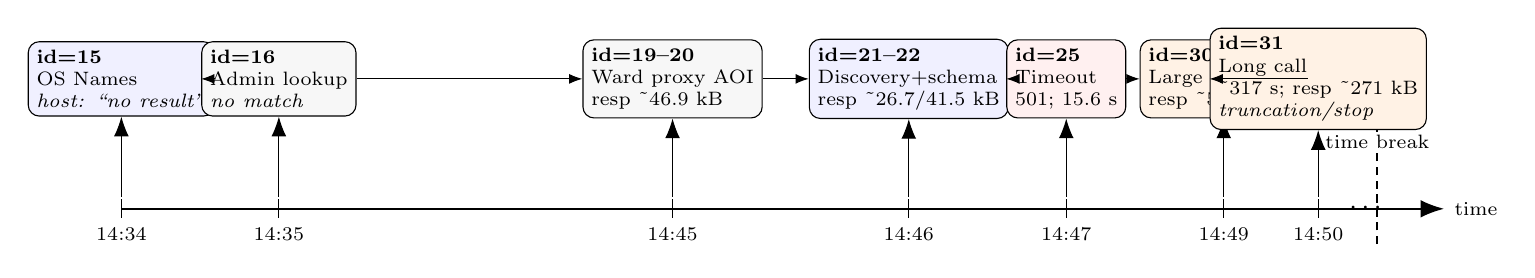
\begin{tikzpicture}[
  x=1cm,y=1cm,
  font=\scriptsize,
  >=Latex,
  event/.style={draw,rounded corners,fill=gray!6,inner sep=3pt,align=left},
  call/.style={draw,rounded corners,fill=blue!6,inner sep=3pt,align=left},
  fail/.style={draw,rounded corners,fill=red!6,inner sep=3pt,align=left},
  heavy/.style={draw,rounded corners,fill=orange!10,inner sep=3pt,align=left},
  axis/.style={draw,thick,-{Latex[length=3mm]}}
]
% timeline axis (taller canvas and explicit break)
\draw[axis] (0,0) -- (16.8,0) node[right]{time};

% ticks (compressed after last call)
\foreach \x/\t in {0/14:34, 2/14:35, 7/14:45, 10/14:46, 12/14:47, 14/14:49, 15.2/14:50} {
  \draw (\x,0.12) -- (\x,-0.12);
\node[below] at (\x,-0.12) {\scriptsize \t};
}
% explicit time-break marker (not to scale)
\draw[densely dashed,thick] (15.95,-0.45) -- (15.95,2.25);
\node[fill=white,inner sep=1pt] at (15.95,0.85) {\scriptsize time break};
\node at (15.8,0) {\normalsize$\cdots$};

% events
\node[call] (e15) at (0,1.65) {\textbf{id=15}\\OS Names\\\textit{host: ``no result''}};
\draw[-{Latex[length=2.5mm]}] (0,0.15) -- (e15.south);

\node[event] (e16) at (2,1.65) {\textbf{id=16}\\Admin lookup\\\textit{no match}};
\draw[-{Latex[length=2.5mm]}] (2,0.15) -- (e16.south);

\node[event] (e19) at (7,1.65) {\textbf{id=19--20}\\Ward proxy AOI\\resp \textasciitilde{}46.9 kB};
\draw[-{Latex[length=2.5mm]}] (7,0.15) -- (e19.south);

\node[call] (e21) at (10,1.65) {\textbf{id=21--22}\\Discovery+schema\\resp \textasciitilde{}26.7/41.5 kB};
\draw[-{Latex[length=2.5mm]}] (10,0.15) -- (e21.south);

\node[fail] (e25) at (12,1.65) {\textbf{id=25}\\Timeout\\501; 15.6 s};
\draw[-{Latex[length=2.5mm]}] (12,0.15) -- (e25.south);

\node[heavy] (e30) at (14,1.65) {\textbf{id=30}\\Large geometry\\resp \textasciitilde{}555 kB};
\draw[-{Latex[length=2.5mm]}] (14,0.15) -- (e30.south);

\node[heavy] (e31) at (15.2,1.65) {\textbf{id=31}\\Long call\\\textasciitilde{}317 s; resp \textasciitilde{}271 kB\\\textit{truncation/stop}};
\draw[-{Latex[length=2.5mm]}] (15.2,0.15) -- (e31.south);

% connectors
\draw[->,thin] (e15.east) -- (e16.west);
\draw[->,thin] (e16.east) -- (e19.west);
\draw[->,thin] (e19.east) -- (e21.west);
\draw[->,thin] (e21.east) -- (e25.west);
\draw[->,thin] (e25.east) -- (e30.west);
\draw[->,thin] (e30.east) -- (e31.west);
\end{tikzpicture}%
}
\caption{Compressed timeline with payload/latency cues (not to scale after 14:50; ellipsis indicates compression).}
\end{figure}

\subsection{Confirmed turning points (discovery → failure → degradation → stop)}

Evidence for turning points is taken from the transcript and tool trace. \cite{artefact_claude_stopped_after_ngd_features_2026_02_18,artefact_codex_trace_jsonl_2026_02_18}

\begin{enumerate}[leftmargin=*]
  \item \textbf{Discovery (but user-visible failure):} \texttt{id=15} succeeded, yet the host indicated “no result received”.
  \item \textbf{Boundary failure:} \texttt{id=16} returned no match; \texttt{id=19–20} fell back to a ward polygon.
  \item \textbf{Degradation:} schema fetch (\texttt{id=22}), upstream timeout (\texttt{id=25}), then geometry-heavy calls (\texttt{id=30}, \texttt{id=31}).
  \item \textbf{Stop (user-visible):} adapter truncation appears before the final “could not be fully generated” marker.
\end{enumerate}

\section{Deliverables and timeline (draft)}

\subsection{Deliverables}
\begin{itemize}[leftmargin=*]
  \item A 6--10 page report (accessible prose, with citations) explaining the model and design patterns.
  \item A case-study appendix summarising the peatmap/audit evidence and the derived requirements.
  \item A slide deck narrative (10--12 slides) plus demo script aligned to the audience outcomes.
  \item A one-page ``assurance questions'' checklist for non-technical leads.
\end{itemize}

\section{Risks and guardrails}

\subsection{Risks}
\begin{itemize}[leftmargin=*]
  \item Over-claiming: confusing information retrieval with grounded, auditable answers.\cite{owasp_llm_top10,ncsc_secure_ai_guidelines}
  \item Safety and privacy: mixed-sensitivity data access without sufficient end-to-end controls.\cite{ico_ai_data_protection,ncsc_secure_ai_guidelines,five_safes_framework}
  \item Trust: inability to explain ``why'' an answer was produced, or to reproduce it later.\cite{prov_o,prov_dm,algorithmic_transparency_recording_standard}
  \item Operational: cost blow-ups, latency, unreliable tool behaviour, and poor degradation modes.\cite{ncsc_secure_ai_guidelines,owasp_llm_top10}
\end{itemize}

\subsection{Guardrails (design commitments)}
\begin{itemize}[leftmargin=*]
  \item Explicit dataset scoping and permissions by default.\cite{five_safes_framework,ico_ai_data_protection}
  \item Provenance-first outputs (sources, transformations, and uncertainty where relevant).\cite{prov_o,prov_dm}
  \item Auditing and monitoring as first-class features.\cite{algorithmic_transparency_recording_standard,ncsc_secure_ai_guidelines}
  \item Progressive disclosure: start simple and safe; expand capability as assurance matures.\cite{data_ai_ethics_framework}
\end{itemize}

\section{Failure taxonomy: MCP-Geo peatland survey incident}

This taxonomy is designed for public-sector MCP servers where tool outputs must be safe, auditable, and reliable under real-time questioning.

\textbf{Primary evidence used:} transcript + tool trace + trace-derived forensic analyses \cite{artefact_claude_stopped_after_ngd_features_2026_02_18,artefact_codex_trace_jsonl_2026_02_18,artefact_floor_question_analysis_2026_02_19,artefact_forensic_study_mcp_geo_2026_02_19}.

Each failure mode includes: \textbf{definition}, \textbf{symptoms}, \textbf{evidence in this case (ids)}, \textbf{impact}, and \textbf{mitigations}. Evidence (ids, payload sizes, latency, and stop markers) is drawn from the tool trace and transcript. \cite{artefact_codex_trace_jsonl_2026_02_18,artefact_claude_stopped_after_ngd_features_2026_02_18}

---

\subsection*{\arabic{section}.F01 Discovery gap (tool routing not aligned to user intent)}

\begin{itemize}[leftmargin=*]
\item \textbf{Definition:} the system fails to route a user’s query to the most appropriate discovery tool(s) for that intent.
\item \textbf{Symptoms:} extra “search” calls, meandering exploration, failure to establish an authoritative area-of-interest quickly.
\item \textbf{Evidence:} \texttt{id=15} used an appropriate tool (OS Names), but the workflow immediately moved to Places/POI (\texttt{id=17–18}) after a host-perceived failure.
\item \textbf{Impact:} slower answers; increased risk of anchoring on the wrong geometry.
\item \textbf{Mitigations:} intent router; tool-choice hints; retry-on-host-mismatch; “names first” policy for landscapes.
\end{itemize}

\subsection*{\arabic{section}.F02 Host–server perception mismatch}

\begin{itemize}[leftmargin=*]
\item \textbf{Definition:} MCP server returns a valid response, but the host/runtime reports it as missing/failed (or vice versa).
\item \textbf{Symptoms:} “No result received…” despite trace indicating 200; sudden pivots.
\item \textbf{Evidence:} \texttt{id=15} success vs transcript error.
\item \textbf{Impact:} incorrect downstream decisions; trust erosion; harder audits (“what really happened?”).
\item \textbf{Mitigations:} end-to-end correlation IDs; host acknowledgement receipts; deterministic replay; tool-result integrity checks.
\end{itemize}

\subsection*{\arabic{section}.F03 Semantic mismatch (using address/POI tools to locate a landscape)}

\begin{itemize}[leftmargin=*]
\item \textbf{Definition:} the wrong class of dataset is queried for the concept in the user’s question.
\item \textbf{Symptoms:} results dominated by addresses, not areas; irrelevant hits.
\item \textbf{Evidence:} Places/POI calls \texttt{id=17–18} produced address-like matches.
\item \textbf{Impact:} wasted calls; incorrect anchors; higher cognitive load for the model/user.
\item \textbf{Mitigations:} schema-level “intended use” metadata; tool router that blocks/penalises known-mismatch paths.
\end{itemize}

\subsection*{\arabic{section}.F04 Missing boundary datasets (designated/protected landscapes absent)}

\begin{itemize}[leftmargin=*]
\item \textbf{Definition:} the server lacks the boundary layers required to resolve common public-sector “named area” queries.
\item \textbf{Symptoms:} falling back to administrative proxies (wards, districts) for non-admin entities.
\item \textbf{Evidence:} \texttt{id=16} no admin match; \texttt{id=19–20} ward geometry used as proxy AOI.
\item \textbf{Impact:} wrong survey extent; high risk of misleading conclusions.
\item \textbf{Mitigations:} add boundary catalogue for AONB/National Landscapes, National Parks, SSSI, SAC/SPA, etc.; provenance labels “authoritative vs proxy”.
\end{itemize}

\subsection*{\arabic{section}.F05 Ontology / attribute mismatch (peat is not reliably represented by land-cover description)}

\begin{itemize}[leftmargin=*]
\item \textbf{Definition:} the attribute(s) used as a proxy do not capture the target phenomenon.
\item \textbf{Symptoms:} “no peat” false negatives; overconfidence from sparse proxies.
\item \textbf{Evidence:} direct \texttt{description="Peat"} filter (\texttt{id=23}) returned zero; later reasoning relied on heath/marsh proxies.
\item \textbf{Impact:} mistaken claims; poor decision support.
\item \textbf{Mitigations:} route to peat-specific authoritative datasets (e.g., England Peat Map) and/or habitat inventories; force “proxy-only” disclaimers when using land-cover.
\end{itemize}

\subsection*{\arabic{section}.F06 Filtering and pagination semantics mismatch (local post-filtering treated as global truth)}

\begin{itemize}[leftmargin=*]
\item \textbf{Definition:} filtering is applied only to the returned page but interpreted as matching the entire universe.
\item \textbf{Symptoms:} “count=0” while the dataset is large; inconsistent counters.
\item \textbf{Evidence:} inconsistencies in \texttt{numberReturned} vs empty \texttt{features} (\texttt{id=23}, \texttt{id=29}).
\item \textbf{Impact:} broken analytics; misleading metrics; brittle automation.
\item \textbf{Mitigations:} explicit “filterApplied: upstream|local”; scan budgets; correct counters; tests for empty results and pagination.
\end{itemize}

\subsection*{\arabic{section}.F07 Upstream reliability / timeout failure}

\begin{itemize}[leftmargin=*]
\item \textbf{Definition:} the upstream service times out or fails under query load.
\item \textbf{Symptoms:} 5xx with timeout; retries; degraded output quality.
\item \textbf{Evidence:} \texttt{id=25} status 501 with \texttt{UPSTREAM\_CONNECT\_ERROR} and \texttt{read timeout=5}.
\item \textbf{Impact:} partial answers; user-visible errors; repeated calls increase pressure further.
\item \textbf{Mitigations:} configurable timeouts; adaptive retries; degrade plan (reduce bbox, drop geometry, lower limit).
\end{itemize}

\subsection*{\arabic{section}.F08 Payload and latency pressure (context bloat)}

\begin{itemize}[leftmargin=*]
\item \textbf{Definition:} large responses and long calls exhaust host/runtime limits, even when the MCP call succeeds.
\item \textbf{Symptoms:} truncation markers; “response could not be fully generated”; sudden stop after heavy results.
\item \textbf{Evidence:} \texttt{id=30} \textasciitilde{}555 kB; \texttt{id=31} \textasciitilde{}317 s latency with \textasciitilde{}271 kB response; transcript truncation then failure marker.
\item \textbf{Impact:} session termination; inability to complete reasoning; audit outputs incomplete.
\item \textbf{Mitigations:} thin defaults; progressive disclosure; resource-backed results; payload thresholds; “counts-first” policies.
\end{itemize}

\subsection*{\arabic{section}.F09 Input validation gaps (silent ignoring of polygon constraints)}

\begin{itemize}[leftmargin=*]
\item \textbf{Definition:} invalid inputs are accepted but ignored without explicit warnings, altering query meaning.
\item \textbf{Symptoms:} polygon supplied but query runs as bbox-only; user believes a constraint applied.
\item \textbf{Evidence:} polygon provided as a JSON string in \texttt{id=30} (likely ignored by parser).
\item \textbf{Impact:} incorrect spatial constraint; larger-than-intended result sets; more payload pressure.
\item \textbf{Mitigations:} strict input typing; reject invalid polygon types; warnings when a constraint is dropped.
\end{itemize}

\subsection*{\arabic{section}.F10 Audit and provenance insufficiency}

\begin{itemize}[leftmargin=*]
\item \textbf{Definition:} outputs do not clearly state boundary sources, dataset limitations, and uncertainty.
\item \textbf{Symptoms:} inability to defend conclusions; hard to replay why a choice was made.
\item \textbf{Evidence:} ward boundary used as proxy without an authoritative AONB boundary available.
\item \textbf{Impact:} reduced decision-quality; governance risk.
\item \textbf{Mitigations:} mandatory provenance block; confidence labels; trace-to-report auto-generation.
\end{itemize}

---

\subsection{How to use this taxonomy}

\begin{itemize}[leftmargin=*]
\item Use \textbf{F1–F4} to assess “can we find the right area and data quickly?”
\item Use \textbf{F5–F6} to assess “are we measuring the right thing, correctly?”
\item Use \textbf{F7–F9} to assess “will it work under pressure?”
\item Use \textbf{F10} to assess “can we defend and audit the answer?”
\end{itemize}

\begin{quote}
\textit{Standards note:} For provenance representations, see W3C PROV-O. \cite{prov_o}\\
\end{quote}

\begin{quote}
\textit{Discovery note:} For catalogue interoperability concepts, see DCAT v3. \cite{dcat3}\\
\end{quote}

\section{Requirements for an MCP “middle layer” in public-sector settings (derived from the case)}

These requirements are written to be \textbf{testable}, \textbf{auditable}, and aligned to public-sector realities (mixed sensitivity, mixed data quality, scrutiny, and real-time questioning).

\textbf{Primary evidence used:} transcript + tool trace + trace-derived forensic analyses \cite{artefact_claude_stopped_after_ngd_features_2026_02_18,artefact_codex_trace_jsonl_2026_02_18,artefact_floor_question_analysis_2026_02_19,artefact_forensic_study_mcp_geo_2026_02_19}.

\textbf{Standards and guidance anchors} used for requirements framing include MCP spec, provenance/catalogue standards, and UK assurance guidance. \cite{mcp_spec_2025_11_25,prov_o,prov_dm,dcat3,ncsc_secure_ai_guidelines,ico_ai_data_protection,data_ai_ethics_framework,five_safes_framework,algorithmic_transparency_recording_standard,owasp_llm_top10}

Each requirement includes an \textbf{acceptance test}.

---

\subsection*{\thesection.R01 Intent routing: map questions to an explicit workflow}
\textbf{Requirement:} The server MUST classify each request into an intent class (e.g., \textit{named-area lookup}, \textit{boundary resolution}, \textit{indicator scan}, \textit{detailed geometry extract}) and route to an explicit workflow with safe defaults. \cite{mcp_spec_2025_11_25,owasp_llm_top10,ncsc_secure_ai_guidelines}

\textbf{Acceptance tests:}
\begin{itemize}[leftmargin=*]
\item Given “peatland site survey … Bowland”, the server selects \textit{environmental survey} intent and triggers \textit{boundary resolution} before any heavy NGD geometry calls.
\item The chosen workflow is recorded in the audit log.
\end{itemize}

\subsection*{\thesection.R02 Boundary catalogue: resolve named landscapes beyond administrative geographies}
\textbf{Requirement:} The server MUST support authoritative boundaries for common designated areas (at minimum: National Landscapes/AONB, National Parks, SSSI; configurable by nation) and MUST label when a proxy boundary is used. \cite{dcat3,data_ai_ethics_framework,algorithmic_transparency_recording_standard}

\textbf{Acceptance tests:}
\begin{itemize}[leftmargin=*]
\item “Forest of Bowland” resolves to an authoritative National Landscape polygon when available.
\item If not available, the output includes \texttt{boundaryType=proxy}, \texttt{proxyReason}, and the exact proxy dataset used.
\end{itemize}

\subsection*{\thesection.R03 “Counts-first” default mode for large-area survey questions}
\textbf{Requirement:} For survey-style questions, the server MUST default to a low-payload indicator scan: \cite{owasp_llm_top10,ncsc_secure_ai_guidelines}
\begin{itemize}[leftmargin=*]
\item \texttt{resultType=hits},
\item \texttt{includeGeometry=false},
\item minimal fields,
\item and spatial tiling if the extent is large.
\end{itemize}

\textbf{Acceptance tests:}
\begin{itemize}[leftmargin=*]
\item A new “survey” request returns an indicator summary without any tool output exceeding a configured size threshold (e.g., 50 kB).
\item Geometry is only fetched after the user or workflow explicitly requests it.
\end{itemize}

\subsection*{\thesection.R04 Payload guardrails with progressive disclosure}
\textbf{Requirement:} The server MUST enforce payload budgets and progressive disclosure: \cite{owasp_llm_top10,ncsc_secure_ai_guidelines}
\begin{itemize}[leftmargin=*]
\item clamp \texttt{limit} to upstream maxima,
\item warn on large bboxes,
\item split requests into tiles/pages,
\item and never stream multi-hundred-kilobyte feature collections inline by default.
\end{itemize}

\textbf{Acceptance tests:}
\begin{itemize}[leftmargin=*]
\item Requests with \texttt{limit>100} are clamped and a warning is returned.
\item Any response >200 kB is converted into a summary + handle (see R5), not inline JSON.
\end{itemize}

\subsection*{\thesection.R05 Resource-backed result delivery for large datasets}
\textbf{Requirement:} When tool outputs exceed a threshold, the server MUST store full results server-side (or in an approved blob store) and return: \cite{mcp_spec_2025_11_25,owasp_llm_top10}
\begin{itemize}[leftmargin=*]
\item a compact summary (counts, bbox, sample IDs), and
\item a stable \texttt{resource://} handle for paging/export.
\end{itemize}

\textbf{Acceptance tests:}
\begin{itemize}[leftmargin=*]
\item The “large geometry” scenario returns a handle and a summary; follow-up “fetch next page” uses the handle without recomputing earlier pages.
\item Resources include TTL and access controls appropriate to data sensitivity.
\end{itemize}

\subsection*{\thesection.R06 Correct and explicit counting semantics}
\textbf{Requirement:} The server MUST provide unambiguous counters: \cite{algorithmic_transparency_recording_standard,prov_dm}
\begin{itemize}[leftmargin=*]
\item \texttt{numberReturned} MUST equal the number of features in \texttt{features[]},
\item \texttt{count} MUST be explicitly defined (returned count vs total matched),
\item and when local filtering is used, the response MUST state \texttt{filterApplied=local} and the scan scope/budget.
\end{itemize}

\textbf{Acceptance tests:}
\begin{itemize}[leftmargin=*]
\item Empty result sets always return \texttt{numberReturned=0}.
\item A regression test covers \texttt{filter}+\texttt{resultType=results} and confirms counters remain consistent.
\end{itemize}

\subsection*{\thesection.R07 Explicit filter model: upstream CQL vs local post-filter}
\textbf{Requirement:} The tool schema MUST distinguish: \cite{prov_dm,algorithmic_transparency_recording_standard,owasp_llm_top10}
\begin{itemize}[leftmargin=*]
\item upstream filters (e.g., CQL, filter-lang),
\item and local post-filters.
\end{itemize}
If local post-filtering is used, the server MUST prevent global claims unless all pages are scanned (or it explicitly marks the result as partial).

\textbf{Acceptance tests:}
\begin{itemize}[leftmargin=*]
\item For a local filter with paging, the response contains \texttt{partialScan=true} unless all pages are scanned within the budget.
\item The report generator refuses to state “no peat present” unless the scan completeness is 100\% or an authoritative peat dataset is used.
\end{itemize}

\subsection*{\thesection.R08 Strict geometry input validation (no silent downgrades)}
\textbf{Requirement:} Any supplied polygon/geometry constraint MUST be validated and either applied or rejected. The server MUST NOT silently ignore a geometry constraint. \cite{ncsc_secure_ai_guidelines,owasp_llm_top10}

\textbf{Acceptance tests:}
\begin{itemize}[leftmargin=*]
\item If \texttt{polygon} is provided as a string (wrong type), the tool returns \texttt{INVALID\_INPUT} with a helpful message.
\item If both bbox and polygon are supplied, the server reports which constraint is applied and why.
\end{itemize}

\subsection*{\thesection.R09 Resilience: adaptive retries and degrade plan for upstream errors}
\textbf{Requirement:} On upstream timeouts or transient errors, the server MUST: \cite{ncsc_secure_ai_guidelines,owasp_llm_top10}
\begin{itemize}[leftmargin=*]
\item retry with exponential backoff (idempotent calls only),
\item and apply a “degrade plan” (reduce bbox, drop geometry, lower limit) before failing.
\end{itemize}

\textbf{Acceptance tests:}
\begin{itemize}[leftmargin=*]
\item In a simulated timeout, the second attempt uses reduced cost parameters and succeeds, with an audit entry describing the degrade plan.
\item The final user output includes which calls were retried and which degradations were applied.
\end{itemize}

\subsection*{\thesection.R10 Provenance-by-default output blocks}
\textbf{Requirement:} Every user-facing answer MUST include a provenance block: \cite{prov_o,prov_dm,algorithmic_transparency_recording_standard,dcat3}
\begin{itemize}[leftmargin=*]
\item datasets used (name, version/date, licensing),
\item boundary source + type (authoritative/proxy),
\item query parameters (bbox/polygon, paging completeness),
\item and explicit limitations.
\end{itemize}

\textbf{Acceptance tests:}
\begin{itemize}[leftmargin=*]
\item Generated answers always include a provenance block, even in “quick answer” mode.
\item Removing the provenance block fails CI for the report generator.
\end{itemize}

\subsection*{\thesection.R11 Sensitivity guardrails and policy-aware redaction}
\textbf{Requirement:} The server MUST support data-classification-aware behaviour: \cite{ico_ai_data_protection,five_safes_framework,data_ai_ethics_framework,ncsc_secure_ai_guidelines}
\begin{itemize}[leftmargin=*]
\item prevent accidental retrieval/exposure of sensitive attributes,
\item redact or aggregate by default,
\item and require explicit privilege and justification for sensitive layers.
\end{itemize}

\textbf{Acceptance tests:}
\begin{itemize}[leftmargin=*]
\item A restricted dataset cannot be accessed without a declared clearance token/role.
\item Responses from restricted datasets are automatically summarised/aggregated and audited.
\end{itemize}

\subsection*{\thesection.R12 Audit-ready observability (trace → report)}
\textbf{Requirement:} The server MUST emit structured audit logs that can be deterministically replayed into a timeline report: \cite{algorithmic_transparency_recording_standard,prov_o,mcp_spec_2025_11_25,ncsc_secure_ai_guidelines}
\begin{itemize}[leftmargin=*]
\item tool calls (args, status, latency, sizes),
\item routing decisions,
\item warnings/guardrails triggered,
\item and resource handles created.
\end{itemize}

\textbf{Acceptance tests:}
\begin{itemize}[leftmargin=*]
\item A report generator can rebuild a timeline table identical (within tolerances) to the runtime record.
\item Correlation IDs link host messages to tool calls, reducing host–server mismatch risk.
\end{itemize}

\textit{Provenance reference:} W3C PROV-O. \cite{prov_o}

\textit{Catalogue reference:} W3C DCAT v3. \cite{dcat3}

\section{Demo script: MCP-Geo as the “middle layer” from apps to answers}

\textbf{Evidence basis for this demo narrative:} transcript + tool trace + trace-derived forensic analyses \cite{artefact_claude_stopped_after_ngd_features_2026_02_18,artefact_codex_trace_jsonl_2026_02_18,artefact_floor_question_analysis_2026_02_19,artefact_forensic_study_mcp_geo_2026_02_19}.

\textbf{Assurance framing references (for Q\&A):} Five Safes, ICO AI \& data protection, NCSC secure AI development guidance, ATRS, OWASP LLM controls, and MCP/provenance standards. \cite{five_safes_framework,ico_ai_data_protection,ncsc_secure_ai_guidelines,algorithmic_transparency_recording_standard,owasp_llm_top10,mcp_spec_2025_11_25,prov_o,dcat3}

Audience: UK Government and wider public sector, mostly non-technical.
Goal: show that MCP lets us shift from \textit{app-centric} integration to \textit{data-to-answers} capability, with governance and safety.

% (visual separator; keep it from appearing as an em-dash paragraph)
\par\medskip\hrule\medskip

\subsection{Setup (before the room)}
\textbf{On screen:}
\begin{itemize}[leftmargin=*]
\item A simple slide with the title: \textbf{From Apps to Answers: Connecting Public Sector Data to AI with MCP}
\item A single diagram: \textit{Data → Information → Answers} (with “MCP middle layer” as the bridge)
\end{itemize}

\textbf{Narration (10–15s):}
\begin{itemize}[leftmargin=*]
\item “Today I’m not demoing a clever app. I’m demoing a capability: connecting intelligence to the data we already hold.”
\end{itemize}

% (visual separator; keep it from appearing as an em-dash paragraph)
\par\medskip\hrule\medskip

\subsection{The story hook (the floor question)}
\textbf{Say:}
\begin{itemize}[leftmargin=*]
\item “Here’s a real question from a previous session: ‘Do a peatland site survey on the forrest of Bowland.’”
\end{itemize}

\textbf{Show:}
\begin{itemize}[leftmargin=*]
\item The line in \texttt{claude-stopped-after-ngd-features.md} where the question appears (and the later ‘don’t use the web’ constraint).
\item Then show a screenshot/clip of the final user-visible failure (“…could not be fully generated”).
\end{itemize}

\textbf{Say:}
\begin{itemize}[leftmargin=*]
\item “This is exactly the kind of moment that matters in the public sector: a live question, a live answer, and scrutiny.”
\end{itemize}

% (visual separator; keep it from appearing as an em-dash paragraph)
\par\medskip\hrule\medskip

\subsection{2) Reconstruct “what actually happened” (trust via audit)}
\textbf{Show (quickly):}
\begin{itemize}[leftmargin=*]
\item The timeline table (ids 15–31) from the forensic write-up.
\item Highlight three moments with a pointer:
\end{itemize}
  1) \texttt{id=15} \textbf{worked} but was perceived as missing by the host
  2) boundary fell back to a \textbf{ward} (proxy)
  3) payload/latency spike (\texttt{id=30}, \texttt{id=31}) before the stop marker

\textbf{Say:}
\begin{itemize}[leftmargin=*]
\item “MCP gives us auditability. We can see exactly which data sources we touched, how long they took, and where things degraded.” \cite{mcp_spec_2025_11_25,prov_o,algorithmic_transparency_recording_standard}
\end{itemize}

% (visual separator; keep it from appearing as an em-dash paragraph)
\par\medskip\hrule\medskip

\subsection{3) The principle: why a “middle layer” matters}
\textbf{Say:}
\begin{itemize}[leftmargin=*]
\item “If you remember one thing: the middle layer is where \textit{data becomes information}.”
\item “APIs give access; MCP can give \textit{governed, intent-aware} access.” \cite{mcp_spec_2025_11_25,ncsc_secure_ai_guidelines,data_ai_ethics_framework}
\end{itemize}

\textbf{Show:}
\begin{itemize}[leftmargin=*]
\item A slide with three boxes:
\end{itemize}
  - \textbf{Data:} raw datasets (OS, ONS, departmental data)
  - \textbf{Middle layer:} routing, boundaries, guardrails, provenance
  - \textbf{Answers:} plain-language responses, reports, maps

% (visual separator; keep it from appearing as an em-dash paragraph)
\par\medskip\hrule\medskip

\subsection{4) Demonstration part A: the “naïve” path (1 minute)}
Purpose: show what happens without the middle layer’s guardrails.

\textbf{Show:}
\begin{itemize}[leftmargin=*]
\item In the console/log viewer: a single large \texttt{os\_features\_query} with geometry and high limit.
\item Point out: “big payload”, “paging”, “timeouts can happen”.
\end{itemize}

\textbf{Say:}
\begin{itemize}[leftmargin=*]
\item “This is what an app-style integration often does: it pulls the data and hopes.”
\end{itemize}

% (visual separator; keep it from appearing as an em-dash paragraph)
\par\medskip\hrule\medskip

\subsection{5) Demonstration part B: the “middle layer” path (3–4 minutes)}
Purpose: show the same question handled with safe defaults and clearer meaning.

\subsubsection{Step B1 — Resolve the area \textit{authoritatively}}
\textbf{Show:}
\begin{itemize}[leftmargin=*]
\item “Resolve named landscape boundary” (AONB/National Landscape) tool or dataset entry.
\item If not implemented yet: show the design stub and explain how it would plug in.
\end{itemize}

\textbf{Say:}
\begin{itemize}[leftmargin=*]
\item “First: define the survey extent. If we can’t get the authoritative boundary, we label the fallback as a proxy.”
\end{itemize}

\subsubsection{Step B2 — Counts-first survey scan}
\textbf{Show:}
\begin{itemize}[leftmargin=*]
\item A lightweight call: \texttt{resultType=hits}, \texttt{includeGeometry=false}.
\item Output: a tiny summary table of peat-indicator classes (counts only).
\end{itemize}

\textbf{Say:}
\begin{itemize}[leftmargin=*]
\item “Second: we ask the data an economical question first. We don’t drag the whole dataset into the chat.”
\end{itemize}

\subsubsection{Step B3 — Controlled enrichment}
\textbf{Show:}
\begin{itemize}[leftmargin=*]
\item Fetch geometry for a \textit{small} subset only.
\item If result is large: show a \texttt{resource://...} handle returned instead of inline payload.
\end{itemize}

\textbf{Say:}
\begin{itemize}[leftmargin=*]
\item “Third: we enrich progressively. The model can ask follow-up questions, but within budgets.”
\end{itemize}

\subsubsection{Step B4 — Provenance block}
\textbf{Show:}
\begin{itemize}[leftmargin=*]
\item A generated “answer” that ends with:
\end{itemize}
  - boundary source and whether it’s authoritative/proxy
  - datasets used
  - completeness (paging)
  - limitations and next steps

\textbf{Say:}
\begin{itemize}[leftmargin=*]
\item “This is what makes it public-sector ready: you can defend the answer.” \cite{prov_o,algorithmic_transparency_recording_standard}
\end{itemize}

% (visual separator; keep it from appearing as an em-dash paragraph)
\par\medskip\hrule\medskip

\subsection{6) How to handle Q\&A (scripted responses)}

\subsubsection{Q: “Why didn’t it just use the peat map?”}
\textbf{Answer:}
\begin{itemize}[leftmargin=*]
\item “Because we didn’t have that boundary/dataset wired in. That’s the point: MCP lets us add authoritative layers and route to them explicitly, rather than hard-coding a single app.”
\end{itemize}

\subsubsection{Q: “Did MCP fail?”}
\textbf{Answer:}
\begin{itemize}[leftmargin=*]
\item “The trace shows the tool calls succeeded through the final step. The visible failure was host pressure after large outputs. The fix is in the middle layer: payload budgets, resource handles, and thin defaults.”
\end{itemize}

\subsubsection{Q: “What about sensitive data?”}
\textbf{Answer:}
\begin{itemize}[leftmargin=*]
\item “Same pattern: the middle layer controls access. It can default to aggregation/redaction, record provenance, and require explicit privilege for sensitive layers.” \cite{ico_ai_data_protection,five_safes_framework,data_ai_ethics_framework}
\end{itemize}

\subsubsection{Q: “Isn’t this just an API?”}
\textbf{Answer:}
\begin{itemize}[leftmargin=*]
\item “APIs are pipes. The middle layer adds: intent routing, policy, provenance, and audit — and it works across many datasets, not one app.” \cite{mcp_spec_2025_11_25,prov_o,algorithmic_transparency_recording_standard}
\end{itemize}

% (visual separator; keep it from appearing as an em-dash paragraph)
\par\medskip\hrule\medskip

\subsection{Close (30 seconds)}
\textbf{Say:}
\begin{itemize}[leftmargin=*]
\item “Public sector is data-rich. The question is whether we can connect it safely to plain-language questions.”
\item “MCP is a way to turn many datasets into a single governed capability: answers, not apps.” \cite{mcp_spec_2025_11_25,data_ai_ethics_framework}
\end{itemize}

\textbf{Show:}
\begin{itemize}[leftmargin=*]
\item A final slide with the 3 takeaways:
\end{itemize}
  1) \textbf{Define the area}
  2) \textbf{Scan cheaply, enrich progressively}
  3) \textbf{Always include provenance and limits}


\bibliographystyle{plain}
\bibliography{references}

\end{document}
